\documentclass[10pt,twocolumn,letterpaper]{article}
\usepackage[italian]{babel} 
\usepackage[utf8]{inputenc} 
\usepackage{cvpr}
\usepackage{times}
\usepackage{epsfig}
\usepackage{graphicx}
\usepackage{amsmath}
\usepackage{amssymb}
\usepackage[Algoritmo]{algorithm}
\usepackage{algpseudocode}

\usepackage{url}

% Include other packages here, before hyperref.

% If you comment hyperref and then uncomment it, you should delete
% egpaper.aux before re-running latex.  (Or just hit 'q' on the first latex
% run, let it finish, and you should be clear).
%\usepackage[pagebackref=true,breaklinks=true,letterpaper=true,colorlinks,bookmarks=false]{hyperref}

\cvprfinalcopy % *** Uncomment this line for the final submission

\def\cvprPaperID{****} % *** Enter the CVPR Paper ID here
\def\httilde{\mbox{\tt\raisebox{-.5ex}{\symbol{126}}}}

% Pages are numbered in submission mode, and unnumbered in camera-ready
\ifcvprfinal\pagestyle{empty}\fi
\begin{document}

%%%%%%%%% TITLE
\title{Implementazione di un sistema di riconoscimento facciale basato sul metodo di Viola e Jones}

\author{Lorenzo Cioni\\
Apprendimento Automatico\\
{\tt\small lore.cioni@gmail.com}}

\maketitle
\thispagestyle{empty}

%%%%%%%%% ABSTRACT
\begin{abstract}
Il riconoscimento facciale gioca un ruolo sempre più determinante in molti settori applicativi, come ad esempio sistemi di sorveglianza, software di editing o applicazioni per l'acquisizione di immagini digitali nei vari dispositivi. In molti casi poi, a causa di alcune specifiche, potrebbe essere necessario dover effettuare dei riconoscimenti in tempo reale, come ad esempio in un video. 
L'obiettivo di questo elaborato è di implementare un sistema di riconoscimento facciale basato sul metodo proposto da P. Viola e M.J. Jones.
\end{abstract}

%-------------------------------------------------------------------------
\section{Introduzione}

Il riconoscimento facciale è stato oggetto di ricerca dai primi anni novanta come parte del ramo del \emph{pattern recognition} e della \emph{object detection}. Il riconoscimento di oggetti e di facce presentano circa gli stessi problemi, ma in particolare, nel secondo caso, i problemi più determinanti sono dati dalla differenza di illuminazione, la scala e la rotazione del volto. 

A questi problemi classici del riconoscimento di oggetti se ne aggiungono altri come la gran varietà di espressioni del volto umano o alla presenza di elementi che ne potrebbero compromettere il riconoscimento, come ad esempio una particolare capigliatura o semplicemente un paio di occhiali.

L'obiettivo di questo elaborato è implementare il metodo di riconoscimento facciale proposto da Viola e Jones \cite{Viola:2004:RRF:966432.966458} e valutarne le criticità e performance.
\section{Il metodo di Viola e Jones}

Il metodo di riconoscimento facciale proposto da Viola e Jones si basa su dei semplici classificatori lineari che operano su delle feature specifiche dell'immagine. Le feature utilizzate sono di tipo binario, molto buone per caratterizzare parti dell'immagine in cui si evidenzia un maggior contrasto: nel caso dei volti queste zone sono tipicamente il naso, gli occhi, etc.

Per consentire di calcolare rapidamente questo tipo di features, Viola e Jones hanno introdotto una nuova rappresentazione dell'immagine chiamata \emph{immagine integrale}. Una volta calcolate queste si procede alla selezione di un loro sottoinsieme utilizzando una versione modificata dell'algoritmo AdaBoost. 

Infine, per la classificazione, viene utilizzata una \emph{cascata di classificatori}. I classificatori sono suddivisi in più livelli rendendo possibile il riconoscimento in tempo reale.
\section{Features}

Uno dei componenti essenziali del metodo di Viola e Jones è l'utilizzo di un sistema di feature molto semplice ed un modo altrettanto veloce per calcolarle.

Viene inizialmente definita una \emph{detection window} di dimensione prefissata (generalmente 24 x 24) e si fa scorrere quest'ultima lungo tutta l'immagine da analizzare alla ricerca di facce. In ciascuna posizione vengono analizzate un'insieme di feature locali, in questo caso le Haar-like.

\subsection{Le features Haar-like}

Le features Haar-like consistono in 2 o più rettangoli bianchi o neri adiacenti all'interno della \emph{detection window}. A partire da una configurazione di rettangoli viene calcolata la differenza delle somme dei pixel sottostanti una regione bianca e quelli sottostanti ad una regione nera. In questo modo è possibile identificare zone in cui vi è un contrasto nella direzione indicata dalla posizione dei rettangoli. Una zona omogenea infatti darà valori circa prossimi a 0.

Sia $X$ un'immagine. Chiamiamo $W$ l'insieme dei pixel sottostanti una regione \textit{bianca} e $B$ l'insieme dei pixel sottostanti una regione \textit{nera}. Il valore della feature è ottenuto tramite

$$
f = \sum_{i \in W} x_i - \sum_{j \in B} x_j
$$

Le features utilizzate nel metodo di Viola e Jones sono di 5 tipi diversi, come mostrato in Figura \ref{fig:haar}.

\begin{figure}[h]
\begin{center}
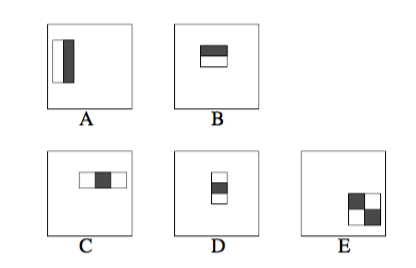
\includegraphics[width=0.35\textwidth]{images/haar}
\end{center}
  \caption{I 5 tipi diversi di Haar-like features utilizzati}
\label{fig:haar}
\end{figure}

Il numero totale di features di tutti e 5 i tipi scalati e traslati all'interno di una \emph{detection window} 24 x 24 è di 162,336. Come nell'implementazione di OpenCV sono state però considerate solo le features con un area superiore a 32 pixels: questo per evitare di andare a considerare delle regioni troppo piccole e irrilevanti ai fini del riconoscimento. Con queste particolari restrizioni il numero totale di features si riduce a 108,490. 

\subsection{Immagini integrali}

Al fine di poter riconoscere i volti in tempo reale è necessario poter valutare queste features in poco tempo. Per fare questo Viola e Jones hanno introdotto una nuova rappresentazione dell'immagine chiamata \emph{immagine integrale}.

L'immagine integrale è costruita utilizzando una matrice della stessa dimensione dell'immagine originale con associata a ciascun elemento la somma dei valori dei pixel che si trovano sopra e a sinistra del pixel corrispondente.

Sia $i$ l'immagine originale e $I$ la sua rappresentazione integrale. Un generico elemento della matrice integrale si trova con:

$$
I(x, y) = \sum_{x' \leq x, y' \leq y} i(x', y')
$$

E' possibile giungere alla costruzione di questa matrice iterativamente utilizzando le seguenti due formule:
$$
s(x, y) = s(x, y - 1) + i(x, y)
$$
$$
I(x, y) = I(x - 1, y) + s(x, y)
$$

\begin{figure}[h]
\begin{center}
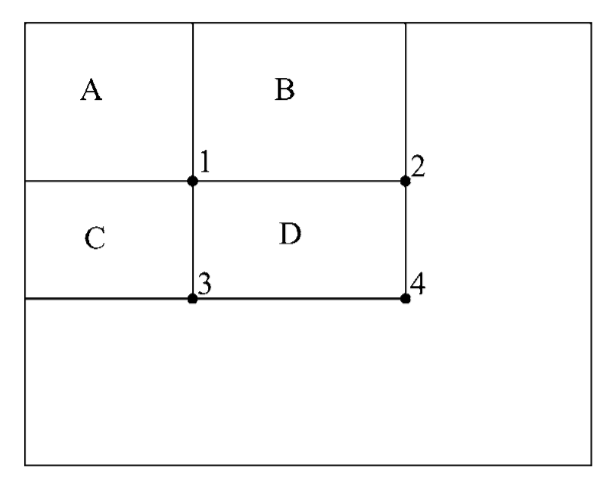
\includegraphics[width=0.35\textwidth]{images/integral}
\end{center}
  \caption{Calcolo della somma dei pixel in una regione rettangolare}
\label{fig:integral}
\end{figure}
A questo punto, data la regione rettangolare $D$, per calcolare la somma dei pixel all'interno della stessa sarà sufficiente valutare
$$
S = I(x_4, y_4) + I(x_1, y_1) - I(x_2, y_2) - I(x_3, y_3)
$$
dunque è un calcolo estremamente veloce.



\section{Boosting}
Una volta estratte le features all'interno di ciascuna detection window si procede con la sua classificazione. Per questa fase vengono usati una serie di semplici classificatori binari basati su una singola feature chiamati \emph{decision stumps}. 

Come visto in precedenza, anche in una finestra relativamente piccola come una detection window 24 x 24, il numero di feature estratte per ciascuna di esse è molto elevato. Nonostante dunque siano molto veloci da calcolare, il tempo necessario sarebbe troppo per applicazioni in tempo reale. 

Si procede dunque alla riduzione dell'insieme delle feature estratte: Viola e Jones utilizzano per questo motivo una versione modificata di AdaBoost per combinare insieme classificatori basati sulle migliori feature selezionate.

\subsection{Decision stumps}

I \emph{decision stumps} sono dei semplici classificatori binari lineari basati su un singolo valore di una feature. 

Un generico classificatore $h$ è definito con una \emph{feature} $f$, una \emph{soglia} $\theta$ ed una \emph{polarità} (\emph{positiva} o  \emph{negativa}). La classificazione è data da:
$$
h(x, f, \theta, p) =
\left\{
\begin{array}{ll}
1 & \mbox{se } p f(x) \leq p \theta \\
-1 & \mbox{altrimenti}
\end{array}
\right.
$$
Questi classificatori sono chiamati \emph{weak classifiers}.

\subsection{AdaBoost}

Gli algoritmi di Boosting combinano insieme una serie di \emph{weak classifiers} per andare a formare uno \emph{strong classifier}. Il metodo standard è l'algoritmo di \emph{AdaBoost} (\emph{Adaptive Boosting}), un algoritmo iterativo che seleziona le features migliori in base ad un errore nei singoli classificatori.

Ad un generico passo dell'algoritmo, la selezione della feature migliore dipende dai risultati della precedente iterazione, dando maggiore enfasi agli esempi che causano un più elevato \emph{error rate}.
Questo è possibile assegnando a ciascun esempio del training set un peso normalizzato (inizialmente uniforme). Ad ogni iterazione dell'algoritmo il peso viene aggiornato per fare in modo di concentrarsi sugli esempi mal classificati nella precedente iterazione. Il risultato di una singola iterazione è la costruzione di un \emph{weak learner} $h_t$. L'errore $\epsilon_t$ del classificatore così definito è dato dalla somma dei pesi degli esempi classificati erroneamente.

Definiamo inizialmente il numero di iterazioni $T$. L'algoritmo di AdaBoost modificato da Viola e Jones è definito come Algoritmo \ref{adaboost}.

Dato $(x_1, y_1), \ldots, (x_{n+m}, y_{n+m})$, con $x \in X$ e $y \in \{-1, 1\}$, $n$ esempi \emph{positivi} e $m$ esempi \emph{negativi}:

\begin{algorithm}
\caption{AdaBoost (Viola e Jones)}\label{adaboost}
\begin{algorithmic}
\State - Inizializza il peso degli esempi positivi a $\frac{1}{2n}$ e quello degli esempi negativi a $\frac{1}{2m}$
\For {$t = 1, \ldots, T$}
\State - Normalizza i pesi così che la loro somma sia unitaria $$w_{i} = \frac{w_{i}}{\sum_{j = 1}^{n+m} w_{j}}$$
\State - Scegli il miglior \emph{weak learner} $h_t$ tale che
$$h_h = \arg \min_{h_j \in H} \epsilon_j \sum_{i = 1}^{n+m} w_{i} [y_i \neq h_j(x_i)]$$
\State - Aggiorna i pesi degli esempi
$$w_i = w_i \beta_{t}^{1 - c_i}$$
dove $\beta_t = \frac{\epsilon_t}{1 - \epsilon_t}$ e $c_i$ vale 1 se l'esempio $i$-esimo è classificato correttamente, altrimenti vale 0
\State - Calcola $\alpha_t = \log (\frac{1}{\beta_t}$
\EndFor
\State - Lo \emph{strong classifier} finale è dato da
$$h(x) = \left\{
\begin{array}{ll}
1 & \mbox{se } \sum_{t = 1}^{T} \alpha_t h_t(x) \geq \frac{1}{2} \sum_{t = 1}^{T} \alpha_t \\
-1 & \mbox{altrimenti}
\end{array}
\right.$$
\end{algorithmic}
\end{algorithm}
La parte $\frac{1}{2} \sum_{t = 1}^{T} \alpha_t$ è detta \emph{soglia} del classificatore, ma si ottengono migliori risultati andando ad aggiustarla successivamente.

\subsection{Scelta del miglior \emph{weak classifier}}

Ad ogni iterazione dell'algoritmo si procede con la selezione della migliore feature che minimizza l'errore dato dalla somma degli esempi classificati erroneamente. Il tempo necessario per questa operazione è $N \times D$, dove $N$ è il numero di esempi e $D$ il numero di features.

Grazie ad una particolare tecnica implementativa, proposta da Viola e Jones nell'articolo, il tempo di calcolo è unica

\subsection{Considerazioni}

Viola e Jones affermano che un classificatore basato su 200 feature estratte giunge ad ottimi risultati in termini di \emph{detection}, ma con un alto costo computazionale che non permette un suo utilizzo in tempo reale, questo a causa del gran numero di feature da calcolare in ciascuna posizione della finestra.

Per ovviare a questo problema è stato proposto un nuovo approccio chiamato \emph{attentional cascade}, in cui una serie di \emph{strong classifiers} sono disposti in cascata in modo tale che siano via via più precisi.
\section{Classificazione}


\subsection{La cascata di classificatori}

\subsection{Post-processing}
\section{Risultati}

\subsection{Creazione del dataset}

\subsection{Esperimenti}


\section{Conclusioni}

%-------------------------------------------------------------------------

{\small
\bibliographystyle{ieee}
\bibliography{egbib}
}

\end{document}
